\documentclass[a4paper,12pt]{article}
\usepackage[utf8]{inputenc}
\usepackage[spanish]{babel}
\usepackage{color}
\usepackage{parskip}
\usepackage{graphicx}
\usepackage{multirow}
\usepackage{listings}
\usepackage{vmargin}
\graphicspath{ {imagenes/} }
\definecolor{mygreen}{rgb}{0,0.6,0}
\definecolor{lbcolor}{rgb}{0.9,0.9,0.9}
\usepackage{epstopdf}


\setpapersize{A4}
\setmargins{2.5cm}       % margen izquierdo
{1.5cm}                        % margen superior
{16.5cm}                      % anchura del texto
{23.42cm}                    % altura del texto
{10pt}                           % altura de los encabezados
{1cm}                           % espacio entre el texto y los encabezados
{0pt}                             % altura del pie de página
{2cm}     

\lstset{
backgroundcolor=\color{lbcolor},
    tabsize=4,    
%   rulecolor=,
    language=[GNU]C++,
        basicstyle=\tiny,
        aboveskip={1.5\baselineskip},
        columns=fixed,
        showstringspaces=false,
        extendedchars=false,
        breaklines=true,
        prebreak = \raisebox{0ex}[0ex][0ex]{\ensuremath{\hookleftarrow}},
        frame=single,
        showtabs=false,
        showspaces=false,
        showstringspaces=false,
        identifierstyle=\ttfamily,
        keywordstyle=\color[rgb]{0,0,1},
        commentstyle=\color[rgb]{0.026,0.112,0.095},
        stringstyle=\color{red},
        numberstyle=\color[rgb]{0.205, 0.142, 0.73},
%        \lstdefinestyle{C++}{language=C++,style=numbers}’.
}

\begin{document}
 \section{Problema}
 Unir dos n árboles binarios utilizando el peso de los nodos.
 \section{Código}
	\subsection{Función Union}
	\begin{lstlisting}
	
void ArbolBinario::uni(list<ArbolBinario>& r){
    FibonacciHeap<NodoDTO> roots;
    for(ArbolBinario ab : r){
        roots.insert(NodoDTO(ab.root));
    }
    if(root){
        roots.insert(NodoDTO(root));
        root = nullptr;
    }
    return _uni(roots);
}

void ArbolBinario::_uni(FibonacciHeap<NodoDTO>& roots){
    if(roots.empty())return;
    if(root == nullptr){
        root = roots.popMin().nodo;
        return _uni(roots);
    }
    Nodo * menor = roots.popMin().nodo;
    Nodo * nuevo = new Nodo(root->valor + menor->valor);
    nuevo->hijos[0] = root;
    nuevo->hijos[1] = menor;
    root = nuevo;
    return _uni(roots);
}
	\end{lstlisting}  
	\subsection{Main}
	\begin{lstlisting}
#include <iostream>
#include "ArbolBinario.h"

using namespace std;

int main()
{
    cout<<"INGRESE SU N"<<endl;
    int n;
    cin>>n;
    ArbolBinario arbolito;
    list<ArbolBinario> arbolitos;
    for(int i = 0; i < n; i++){
        cout<<"CUANTOS NODOS TENDRA EL ARBOL"<<i+1<<"??"<<endl;
        int n2;
        cin>>n2;
        ArbolBinario temp;
        for(int j = 0; j < n2; j++){
            cout<<"INGRESE EL NODO "<<j +1<<endl;
            int val;
            cin>>val;
            temp.insert(val);
        }
        arbolitos.push_back(temp);
    }
    arbolito.uni(arbolitos);
    arbolito.print();
}	
	\end{lstlisting}
	\section{Ejemplo}
	Para el ejemplo ingreso un n = 3.
	El primer arbol, mirando por amplitud, es: 4,3,10.
	El segundo arbol: 6.
	El tercer arbol: 11,1,18,15.
	\begin{figure}[h]
	\centering
	\includegraphics[scale = 0.5]{consol.eps}
	\caption{Consola del programa}
	\end{figure}	
	\begin{figure}[h]
	 \centering
	 
\includegraphics[scale = 0.5]{eje.pdf}
	 \caption{Arbol Resultante}
	\end{figure}

	
\end{document}

